\documentclass[
  bibliography=totoc,     % Literatur im Inhaltsverzeichnis
  captions=tableheading,  % Tabellenüberschriften
  titlepage=firstiscover, % Titelseite ist Deckblatt
]{scrartcl}

% Paket float verbessern
\usepackage{scrhack}

% Warnung, falls nochmal kompiliert werden muss
\usepackage[aux]{rerunfilecheck}

% unverzichtbare Mathe-Befehle
\usepackage{amsmath}
% viele Mathe-Symbole
\usepackage{amssymb}
% Erweiterungen für amsmath
\usepackage{mathtools}

% Fonteinstellungen
\usepackage{fontspec}
% Latin Modern Fonts werden automatisch geladen
% Alternativ:
%\setromanfont{Libertinus Serif}
%\setsansfont{Libertinus Sans}
%\setmonofont{Libertinus Mono}
\recalctypearea % Wenn man andere Schriftarten gesetzt hat,
% sollte man das Seiten-Layout neu berechnen lassen

% deutsche Spracheinstellungen
\usepackage{polyglossia}
\setmainlanguage{german}


\usepackage[
  math-style=ISO,    % ┐
  bold-style=ISO,    % │
  sans-style=italic, % │ ISO-Standard folgen
  nabla=upright,     % │
  partial=upright,   % ┘
  warnings-off={           % ┐
    mathtools-colon,       % │ unnötige Warnungen ausschalten
    mathtools-overbracket, % │
},                       % ┘
]{unicode-math}

% traditionelle Fonts für Mathematik
\setmathfont{Latin Modern Math}
% Alternativ:
%\setmathfont{Libertinus Math}

\setmathfont{XITS Math}[range={scr, bfscr}]
\setmathfont{XITS Math}[range={cal, bfcal}, StylisticSet=1]

% Zahlen und Einheiten
\usepackage[
locale=DE,                   % deutsche Einstellungen
separate-uncertainty=true,   % immer Fehler mit \pm
per-mode=symbol-or-fraction, % / in inline math, fraction in display math
]{siunitx}

% chemische Formeln
\usepackage[
version=4,
math-greek=default, % ┐ mit unicode-math zusammenarbeiten
text-greek=default, % ┘
]{mhchem}

% richtige Anführungszeichen
\usepackage[autostyle]{csquotes}

% schöne Brüche im Text
\usepackage{xfrac}

% Standardplatzierung für Floats einstellen
\usepackage{float}
\floatplacement{figure}{htbp}
\floatplacement{table}{htbp}

% Floats innerhalb einer Section halten
\usepackage[
section, % Floats innerhalb der Section halten
below,   % unterhalb der Section aber auf der selben Seite ist ok
]{placeins}

% Seite drehen für breite Tabellen: landscape Umgebung
\usepackage{pdflscape}

% Captions schöner machen.
\usepackage[
  labelfont=bf,        % Tabelle x: Abbildung y: ist jetzt fett
  font=small,          % Schrift etwas kleiner als Dokument
  width=0.9\textwidth, % maximale Breite einer Caption schmaler
]{caption}
% subfigure, subtable, subref
\usepackage{subcaption}

% Grafiken können eingebunden werden
\usepackage{graphicx}
% größere Variation von Dateinamen möglich
\usepackage{grffile}

% schöne Tabellen
\usepackage{booktabs}

% Verbesserungen am Schriftbild
\usepackage{microtype}

% Literaturverzeichnis
\usepackage[style=alphabetic,]{biblatex}
% Quellendatenbank
\addbibresource{lit.bib}

% Hyperlinks im Dokument
\usepackage[
  unicode,        % Unicode in PDF-Attributen erlauben
  pdfusetitle,    % Titel, Autoren und Datum als PDF-Attribute
  pdfcreator={},  % ┐ PDF-Attribute säubern
  pdfproducer={}, % ┘
]{hyperref}
% erweiterte Bookmarks im PDF
\usepackage{bookmark}

% Trennung von Wörtern mit Strichen
\usepackage[shortcuts]{extdash}

\title{V354: Gedämpfte und erzwungene Schwingungen}
\author{
  Simon Schulte
  \texorpdfstring{
    \\
    \href{mailto:simon.schulte@udo.edu}{simon.schulte@udo.edu}
  }{}
  \texorpdfstring{\and}{, }
  Tim Sedlaczek
  \texorpdfstring{
    \\
    \href{mailto:tim.sedlaczek@udo.edu}{tim.sedlaczek@udo.edu}
  }{}
}
\publishers{TU Dortmund – Fakultät Physik}

\date{Durchführung: 24.01.2017\\
      Abgabe: 31.01.2016}


\begin{document}

\maketitle
\thispagestyle{empty}
\tableofcontents
\newpage
\section{Zielsetzung}
\label{sec:zielsetzung}
Ziel des Versuchs ist die Untersuchung eines gedämpften elektrischen
RCL-Schwingkreises.
\section{Theorie}
\label{sec:theorie}
\subsection{Gedämpfte Schwingung}
\label{sub:gedämpft}
\begin{figure}[htb]
  \centering
  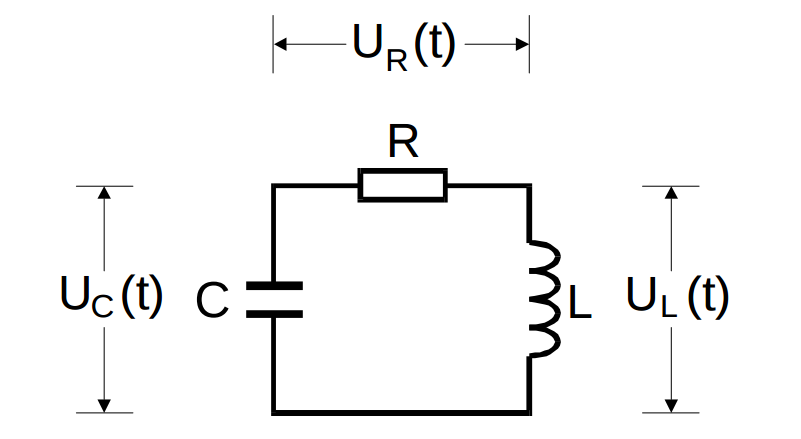
\includegraphics[width=0.75\textwidth]{V3541.png}
  \caption{Der Aufbau eines gedämpften Schwingkreises \cite{anleitung}.}
  \label{fig:V3541}
\end{figure}
In Abbildung \ref{fig:V3541} zu sehen ist der Aufbau eines elektrischen
Schwingkreises. Dieser ist in der Lage nach kurzer Anregung Energie entweder
im magnetischen Feld der Spule oder im elektrischen Feld des Kondensators zu
speichern. Er besteht aus einer Kapazität $C$, einer Induktivität $L$ und einem
ohmschen Widerstand $R$. Die Energie schwingt periodisch zwischen den beiden
Energiereservoirs. Logischerweise ändert der Strom dabei auch seine Richtung.
Die Schwingung kommt irgendwann zum Erliegen, da über den ohmschen Wiederstand
$R$ stets Energie in Form von Wärme verloren geht. Durch diesen Widerstand
entsteht dabei eine kontinuierliche Dämpfung. \\
\\
Das Zeitgesetz lässt sich aus dem 2. Kirchhoffschen Gesetz herleiten.
Es macht eine Aussage über die Amplitude der Kondensatorspannung. Es gilt:
\begin{equation}
    U_{\mathup{R}}(t)+U_{\mathup{C}}(t)+U_{\mathup{L}}(t)=0.
    \label{eqn:kirchhoff}
\end{equation}
Daraus folgt die Differentialgleichung
\begin{equation}
    \frac{\mathup{d}^2}{\mathup{d}t^2}I(t)+\frac{R}{L}\frac{\mathup{d}}{\mathup{d}t}I(t)+\frac{1}{LC}I(t)=0.
    \label{eqn:dgl}
\end{equation}
Die Lösung dieser gewöhnlichen homogenen DGL 2. Ordnung erfolgt über den
komplexen Ansatz:
\begin{equation}
    I(t)=A\mathup{e}^{\mathup{i}\omega t}.
    \label{eqn:ansatz}
\end{equation}
Dieser führt durch Einsetzen, Kürzen und Zusammenfassen zu einem wichtigen
Ausdruck für den Parameter $\omega$:
\begin{equation}
    \omega_{1,2}=\mathup{i}\frac{R}{2L}\pm\sqrt{\frac{1}{LC}-\frac{R^2}{4L^2}}.
    \label{eqn:omega}
\end{equation}
Unter Zuhilfenahme der Abkürzungen
\begin{align}
    2\pi\mu&:=\frac{R}{2L} & 2\pi\nu&:=\sqrt{\frac{1}{LC}-\frac{R^2}{4L^2}}
    \label{eqn:abkuerzungen}
\end{align}
ergibt sich die allgemeine Lösung von Gleichung \eqref{eqn:dgl} als
\begin{equation}
    I(t)=\mathup{e}^{-2\pi\mu t}\left(A_1\mathup{e}^{\mathup{i}2\pi\nu t}+A_2\mathup{e}^{-\mathup{i}2\pi\nu t}\right).
    \label{eqn:allgemeine_loesung}
\end{equation}
Eine Betrachtung der Lösungen \eqref{eqn:allgemeine_loesung} unter physikalischen
Gesichtspunkten ergibt im Wesentlichen zwei zu unterscheidende Fälle mit einem
Spezialfall:\\
\\
Für den ersten Fall: $\frac{1}{LC}>\frac{R^2}{4L^2}$ \\
\\
In diesem Fall ist $\nu$ reell; es existieren weiterhin imaginäre Exponenten in
der Lösungsfunktion $I(t)$. Damit hat die Lösung die Form einer Schwingung mit
exponentiellem Dämpfungsterm, die sich als
\begin{equation}
    I(t)=A_0\mathup{e}^{-2\pi\mu t}\cos{\left(2\pi\nu t+\eta\right)}
    \label{eqn:schwingfall}
\end{equation}
schreiben lässt. $\eta$ bezeichnet hierbei eine Phasenverschiebung, die neben
der Anfangsauslenkung $A_0$ durch die Anfangsbedingungen festgelegt wird. Die
Schwingungsdauer $T$ des Oszillators ergibt sich zu
\begin{equation}
    T=\frac{1}{\nu}=\frac{2\pi}{\sqrt{\frac{1}{LC}-\frac{R^2}{4L^2}}}.
    \label{eqn:schwingungsdauer}
\end{equation}
Eine weitere wichtige Größe in diesem Zusammenhang ist die sogenannte
Abklingdauer $T_{\mathup{ex}}$. Sie gibt die Zeit an, nach welcher die Amplitude
der Schwingung nur noch den $\mathup{e}$-ten Teil ihres Ausgangswertes angenommen hat:
\begin{equation}
    T_{\mathup{ex}}:=\frac{1}{2\pi\mu}=\frac{2L}{R}.
    \label{eqn:abklingdauer}
\end{equation}\\
\\
Für den zweiten Fall: $\frac{1}{LC}<\frac{R^2}{4L^2}$ \\
\\
Tritt dieser Fall ein, so ist $\nu$ imaginär, was zur Folge hat, dass alle
Exponenten der Lösungsfunktion rein reell werden. Daraus folgt, dass
physikalisch betrachtet keine gedämpfte Schwingung sondern eine Relaxation
vorliegt, wobei die Spannung noch maximal ein lokales Extremum annehmen kann.\\
\\
Für den Spezialfall: $\frac{1}{LC}=\frac{R^2}{4L^2}$ \\
\\
In diesem Fall ist $\nu=0$. Die Lösungsfunktion $I(t)$ wird dann zu
\begin{equation}
    I(t)=A\mathup{e}^{-\frac{R}{2L}t}=A\mathup{e}^{-\frac{t}{\sqrt{LC}}}.
    \label{eqn:grenzfall}
\end{equation}
Für diesen, auch als aperiodischen Grenzfall bezeichneten Fall, geht die Spannung
auf schnellstem Weg, ohne ein lokales Extremum anzunehmen, gegen Null.
\subsection{Erzwungene Schwingung}
\label{sub:erzwungen}
\begin{figure}[htb]
  \centering
  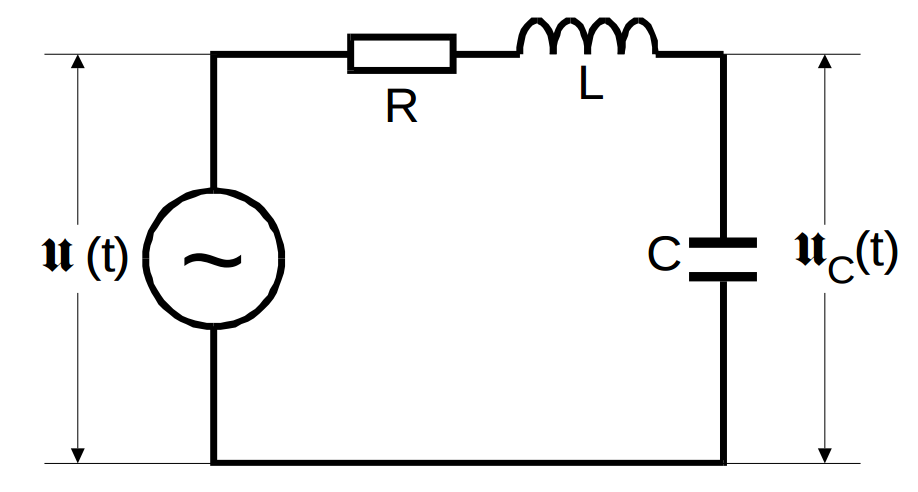
\includegraphics[width=0.75\textwidth]{V3542.png}
  \caption{Der Aufbau eines gedämpften Schwingkreises mit periodischer Anregung \cite{anleitung}.}
  \label{fig:V3542}
\end{figure}
Wenn man nun eine weitere Spannungsquelle an den Schwingkreis anschließt, die
eine Sinusspannung liefert, ergibt sich eine neue DGL aus den Kirchhoffschen Regeln:
\begin{equation}
    LC\frac{\mathup{d}^2}{\mathup{d}t^2}U_{\mathup{C}}(t)+RC\frac{\mathup{d}}{\mathup{d}t}U_{\mathup{C}}(t)+U_{\mathup{C}}(t)=U_0\mathup{e}^{\mathup{i}\omega t}.
    \label{eqn:dgl2}
\end{equation}
Dabei ist $U_\mathup{C}$ die Spannung am Kondensator. Mit dem gleichen Ansatz wie in
\eqref{eqn:ansatz} folgt:
\begin{equation}
    \varphi(\omega)=\arctan\left(\frac{-\omega RC}{1-LC\omega^2}\right).
    \label{eqn:phase}
\end{equation}
Dabei ist allerdings $A$ nun abhängig von $\omega$ und eine komplexe Zahl $A(\omega)$.
$\phi$ ist die Phasenverschiebung zwischen Kondensator- und Erregerspannung.
Für die von $\omega$ abhängige Spannungsamplitude am Kondensator folgt:
\begin{equation}
    U_{\mathup{C}}(\omega)=\frac{U_0}{\sqrt{\left(1-LC\omega^2\right)^2+\omega^2R^2C^2}}.
    \label{eqn:amplitude}
\end{equation}
Während die Spannungsamplitude für $\omega\rightarrow\infty$ gegen Null und für
$\omega\rightarrow 0$ gegen $U_0$ strebt, erreicht sie bei Einstellung der
sogenannten Resonanzfrequenz $\omega_{\mathup{res}}$ einen Wert der größer als
$U_0$ ist. Für die Resonanzfrequenz folgt:
\begin{equation}
    \omega_{\mathup{res}}=\sqrt{\frac{1}{LC}-\frac{R^2}{2L^2}}.
    \label{eqn:resonanz}
\end{equation}
Bei einer schwachen Dämpfung wird die Kondensatorspannung bei dieser Frequenz um
den Faktor
\begin{equation}
    q=\frac{U_\mathup{C, max}}{U_0}=\frac{1}{\omega_0RC}=\frac{1}{R}\sqrt{\frac{L}{C}}U_0
    \label{eqn:guete}
\end{equation}
im Bezug auf die Erregerspannung vergrößert. $q$ ist dabei die Güte. Die Resonanz
eines Schwingkreises ist definiert durch die Breite des Bereichs zwischen den
beiden Frequenzen, bei denen die Spannung bei einer Resonanzfrequenz auf den
$\sfrac{1}{\sqrt{2}}$-ten Teil gefallen ist. Für $\sfrac{R^2}{L^2}\ll\omega_0^2$
gilt näherungsweise:
\begin{equation}
    \omega_+-\omega_-\approx\frac{R}{L}.
    \label{eqn:breite}
\end{equation}
Für die Phasenverschiebung ergeben sich drei Orientierungsgrößen $\omega_0$, $\omega_1$
und $\omega_2$.
$\omega_0$ ist nach
\begin{equation}
  \omega_0 = \sqrt{\frac{1}{LC}}
  \label{eqn:phasepi2}
\end{equation}
definiert. Dort beträgt die Phasenverschiebung $\frac{\pi}{2}$.
Bei $\omega_1$ und $\omega_2$, welche sich nach
\begin{equation}
  \omega_{1,2} = \pm \frac{R}{2L} + \sqrt{\frac{R^2}{4L^2}+\frac{1}{LC}}
  \label{eqn:phase134pi}
\end{equation}
berechnen liegt eine Phase von $\frac{\pi}{4}$ bzw. $\frac{3\pi}{4}$ vor.
\clearpage
\section{Versuchsaufbau}
\label{sec:versuchsaufbau}
\begin{figure}[htb]
  \centering
  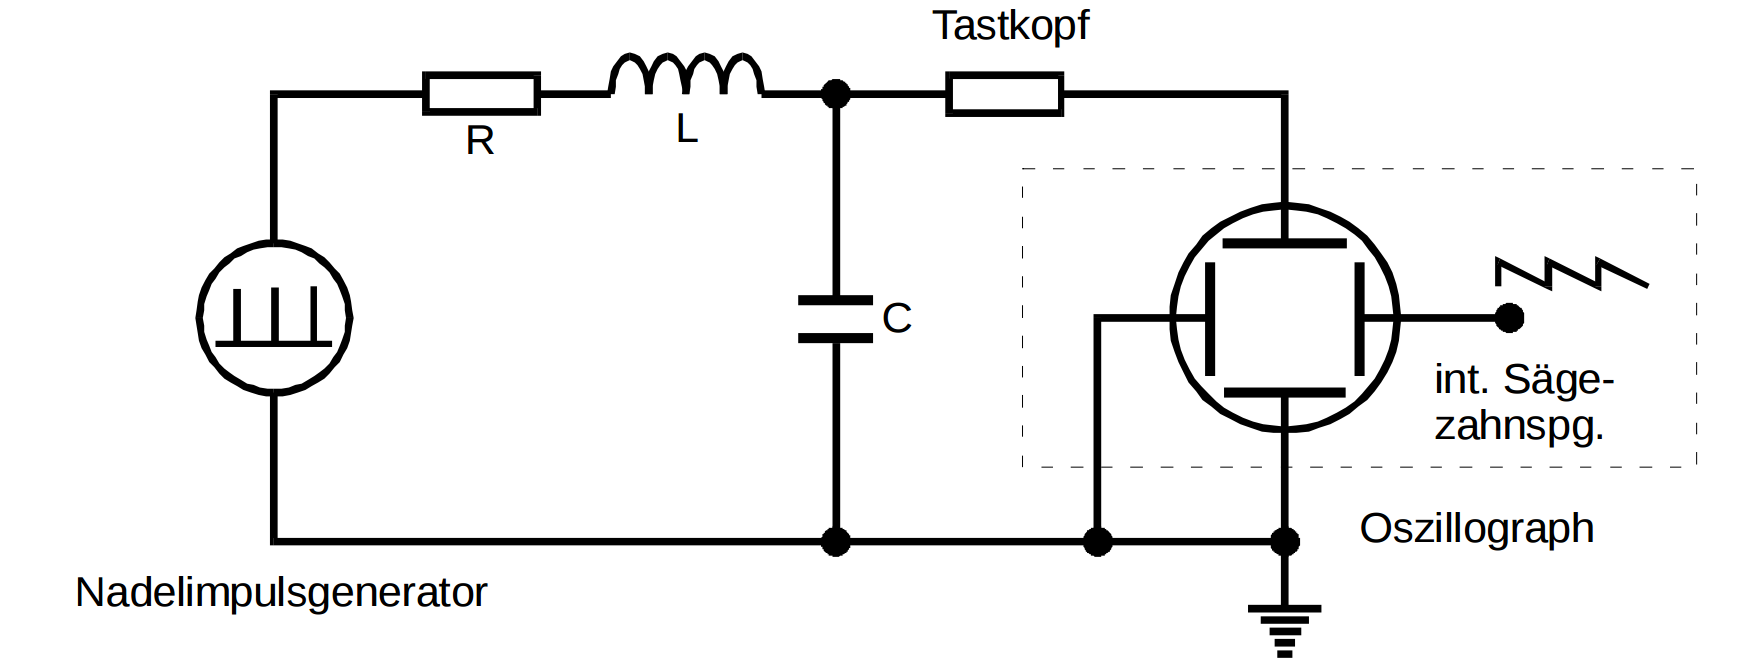
\includegraphics[width=\textwidth]{V3543.png}
  \caption{Versuchsaufbau zur Untersuchung der Kondensatoramplitude eines gedämpften Schwingkreises \cite{anleitung}.}
  \label{fig:V3543}
\end{figure}
\section{Durchführung}
\label{sec:durchführung}
Der Versuch besteht aus 4 Teilversuchen, dabei werden ein Funktionsgenerator,
ein Speicheroszilloskop und ein RCL-Kreis verwendet. Bei dem RCL-Kreis besteht
die Möglichkeit über verschiedene Anschlüsse zwischen einem variablen Widerstand
und zwei festen Widerständen, $R_1$ und $R_2$, zu wählen. \\
\\
Als erstes wird versucht aus der Untersuchung der Kondensatoramplitude eines
gedämpften Schwingkreises dessen Dämpfungswiderstand $R_\mathup{eff}$ zu bestimmen.
Der dafür genutzte Versuchsaufbau ist in Abbildung \ref{fig:V3543} zu sehen. Der Rechteckgenerator
liefert die gedämpften Schwingungen des RCL-Kreises, diese sind auf einem
Oszilloskop zu sehen. Die Generatorfrequenz ist dabei \SI{1468}{\hertz} und es wird $R_1$ verwendet. \\
\\
Als nächstes soll der Widerstand $R_\mathup{ap}$ gefunden werden, bei dem die Dämpfung
genau so stark ist, dass der aperiodische Grenzfall eintritt. Dort wird dann
der variable Widerstand genutzt. Dieser ersetzt dann den Widerstand $R_1$. Es
wird solange der Widerstand $R_\mathup{ap}$ variiert, bis der Wert erreicht ist, an dem
kein lokales Spannungsextremum existiert, sondern die Spannung auf 0 gedämpft
wird. \\
\\
Zur Untersuchung der Frequenzabhängigkeit des RCL-Kreises wird zunächst die
Kondensatorspannung beobachtet. Hier wird nun der vorher verwendete Widerstand
mit dem Widerstand $R_2$ ersetzt. Der RCL-Kreis wird jetzt über einen
frequenzvariablen Sinusgenerator angeregt und die Kondensatorspannung sowie die
Generatorspannung werden nebeneinander dargestellt. Es werden in dem
Frequenzspektrum \SI{4.183}{\kilo\hertz} bis \SI{100}{\kilo\hertz} 15 Messwerte
aufgenommen. Dabei ist Generatorspannung $U_0=\SI{10}{\volt}$ und es werden Werte
für die Kondensatorspannung $U_\mathup{C}$ aufgenommen.\\
\\
Zuletzt wird die Frequenzabhängigkeit der Phasenverschiebung zwischen
Kondensator und Generatorspannung beobachtet. Dabei wird die Phasendifferenz
zwischen $U_0$ und $U_\mathup{C}$ untersucht. Der Ablauf verläuft so, wie
bei der Messung der Abhängigkeit der Spannung.\\
\\
Die Daten des verwendeten Geräts sind:
\begin{align}
  L&=\SI{10.11(3)}{\milli\henry} & C&=\SI{2.098(6)}{\nano\farad}\\
  R_1&=\SI{48.1(1)}{\ohm} & R_2&=\SI{509.5(5)}{\ohm}
\end{align}
\clearpage
\section{Auswertung}
\label{sec:auswertung}
\subsection{Gedämpfte Schwingung}
\begin{figure}[htb]
  \centering
  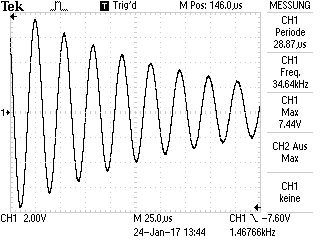
\includegraphics[width=\textwidth]{F0005TEK.jpg}
  \caption{Bildschirmabbild des Oszilloskops von der gedämpften Schwingung.}
  \label{fig:gedämpft}
\end{figure}
In Abbildung \ref{fig:gedämpft} ist das Bild von der gedämpften Schwingung zu sehen.
An diesem wurden die Extrema der Schwingung ausgemessen und damit jeweils die Spannungsamplitude
$U_C$ gegen die Zeit aufgetragen. Die gemessenen Werte stehen in Tabelle \ref{tab:messwerte1}.\\

Zudem wurde nach der Funktion
\begin{equation}
  f \left( t \right) = a \cdot \exp \left( -b \cdot t \right)
  \label{eqn:fit}
\end{equation}
eine Ausgleichskurve bestimmt.
Die entsprechenden Parameter sind:
\begin{align}
  a &= \SI{82(1)}{\volt} & b &= \SI{5596(173)}{\second\tothe{-1}}
\end{align}
Der Graph dazu ist in Abbildung \ref{fig:plot1} zu sehen.
\begin{table}
  \centering
  \caption{Gemessene Amplituden der gedämpften Schwingung.}
  \label{tab:messwerte1}
  \sisetup{table-format=3.2}
  \begin{tabular}{S S[table-format=2.1]}
    \toprule
    {$t \,/\, \si{\micro\second}$} & {$U_C \,/\, \si{\volt}$}\\
    \midrule
    10 & 76\\
    25 & 74\\
    39 & 65\\
    54 & 64\\
    67.5 & 56\\
    82.5 & 54\\
    96.25 & 44\\
    111.25 & 43.6\\
    126 & 40\\
    140 & 36\\
    155 & 34\\
    169 & 34\\
    183 & 30\\
    197.5 & 30\\
    212.5 & 24\\
    227.5 & 24\\
    241.25 & 20\\
    \bottomrule
  \end{tabular}
\end{table}
\clearpage
\begin{figure}[htb]
  \centering
  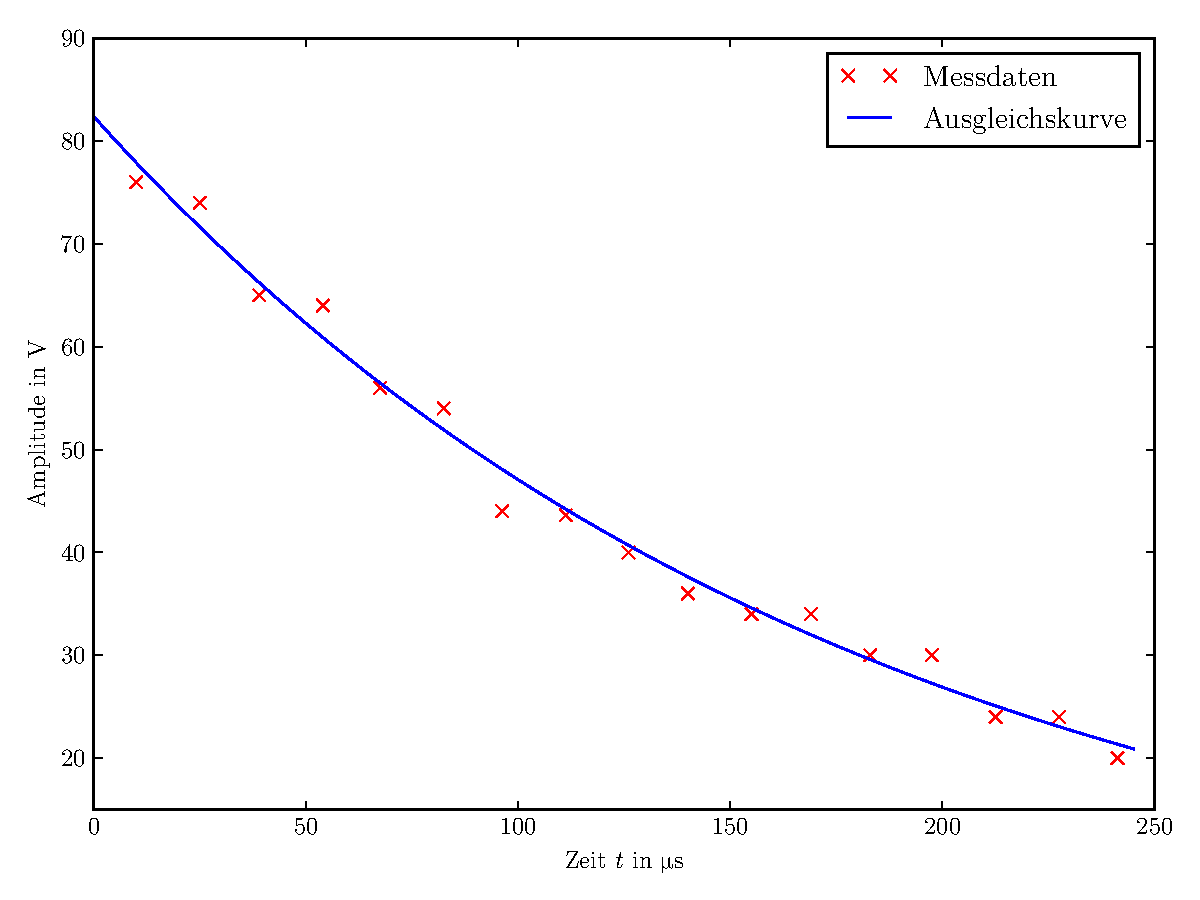
\includegraphics[width=\textwidth]{Plot.pdf}
  \caption{Amplituden der Schwingung in Abhängigkeit von der Zeit.}
  \label{fig:plot1}
\end{figure}
Der so bestimmte Exponent entspricht dem $2\pi\mu$ in den Formeln \eqref{eqn:schwingfall}
und \eqref{eqn:abklingdauer}.
Daraus folgt die Abklingdauer der Schwingung zu
\begin{equation}
  T_\mathup{ex} = \SI{179(6)}{\micro\second}
\end{equation}
und der effektive Widerstand, durch multiplizieren mit der zweifachen Induktivität,
der eingebauten Spule zu
\begin{equation}
  R_\mathup{eff} = \SI{113(4)}{\ohm}.
\end{equation}
\clearpage
\subsection{Aperiodischer Grenzfall}
In Abbildung \ref{fig:apgrenze} ist der Verlauf der Spannung beim aperiodischen
Grenzfall zu sehen. Der hierzu eingestellte Widerstand beträgt
\begin{equation}
  R = \SI{3600}{\ohm}.
\end{equation}
Rechnerisch ergibt sich der Wert, mit der Bedingung für den aperiodischen Grenzfall,
nach
\begin{equation}
  R_\mathup{ap} = 2 \sqrt{\frac{L}{C}}
\end{equation}
zu
\begin{equation}
  R_\mathup{ap} = \SI{4390(9)}{\ohm}.
\end{equation}
\begin{figure}[htb]
  \centering
  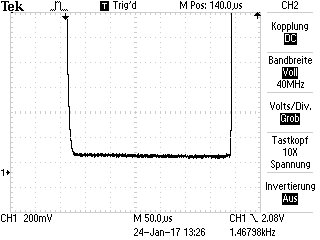
\includegraphics[width=\textwidth]{F0004TEK.jpg}
  \caption{Bildschirmabbild des Oszilloskops vom aperiodischen Grenzfall.}
  \label{fig:apgrenze}
\end{figure}
\clearpage
\subsection{Frequenzabhängigkeit der Spannung am Kondensator und der Phase}
Die mit der Cursor-Funktion des Oszilloskops bestimmten Werte stehen in Tabelle
\ref{tab:messwerte2}.
\begin{table}
  \centering
  \caption{Werte der Spannung, sowie der Phasenverschiebung.}
  \label{tab:messwerte2}
  \sisetup{table-format=3.3}
  \begin{tabular}{S S[table-format=2.2] S[table-format=1.3]}
    \toprule
    {Frequenz $\nu$ des}\\ {Generators in $\si{\kilo\hertz}$} & {$\increment t \,/\, \si{\micro\second}$} & {$\frac{U_\mathup{C}}{U}$}\\
    \midrule
    4.183 & 1.24 & 1\\
    10 & 1.31 & 1.08\\
    20 & 1.4 & 1.44\\
    24 & 1.64 & 1.8\\
    28 & 2.29 & 2.6\\
    32 & 4.41 & 3.6\\
    33 & 6.5 & 3.62\\
    34 & 7.4 & 3.7\\
    35 & 8.3 & 3.62\\
    36 & 9 & 3.4\\
    40 & 10 & 1.92\\
    44 & 9.9 & 1.25\\
    48 & 9.35 & 0.9\\
    60 & 7.9 & 0.45\\
    100 & 5.4 & 0.108\\
    \bottomrule
  \end{tabular}
\end{table}\\
Zur bestimmung der Frequenzabhängigkeit der Spannung am
Kondensator wird der Quotient $\frac{U_\mathup{C}}{U}$ gegen die Frequenz $\nu$
einmal halblogarithmisch (Abbildung \ref{fig:plot2}) und einmal linear (Abbildung \ref{fig:plot3})
aufgetragen. Dabei ist $U$ die Amplitude der Generatorspannung. Aus dem Graphen
wird dann die Resonanzüberhöhung $q$ entnommen.\\

Das Maximum befindet sich bei einer Freqenz von $\SI{33.5}{\kilo\hertz}$ und beträgt
$\SI{37}{\volt}$. Der theoretische Wert für die Resonanzfrequenz berechnet sich nach
Formel \eqref{eqn:resonanz} zu
\begin{equation}
  \nu_\mathup{res} = \SI{34.1}{\kilo\hertz}.
\end{equation}
Damit ergibt sich für die Güte/Resonanzüberhöhung:
\begin{equation}
  q = 3.7
\end{equation}

Geometrisch werden nun die Frequenzen $\nu_+$ und $\nu_-$ bestimmt bzw. abgeschätzt.
Sie liegen bei
\begin{align}
  \nu_- &= \SI{28}{\kilo\hertz} & &\text{und} & \nu_+ &= \SI{38}{\kilo\hertz}.
\end{align}
Die Breite der Resonanzkurve beträgt damit
\begin{equation}
  \nu_+ - \nu_- = \SI{10}{\kilo\hertz}.
\end{equation}

Mit Formel \eqref{eqn:guete} ergibt sich für die Güte ein Wert von
\begin{equation}
  q = 4.3
\end{equation}
und nach \eqref{eqn:breite} für die Breite ein Wert von ca.
\begin{equation}
  \nu_+ - \nu_- = \SI{8}{\kilo\hertz}.
\end{equation}
\begin{figure}[htb]
  \centering
  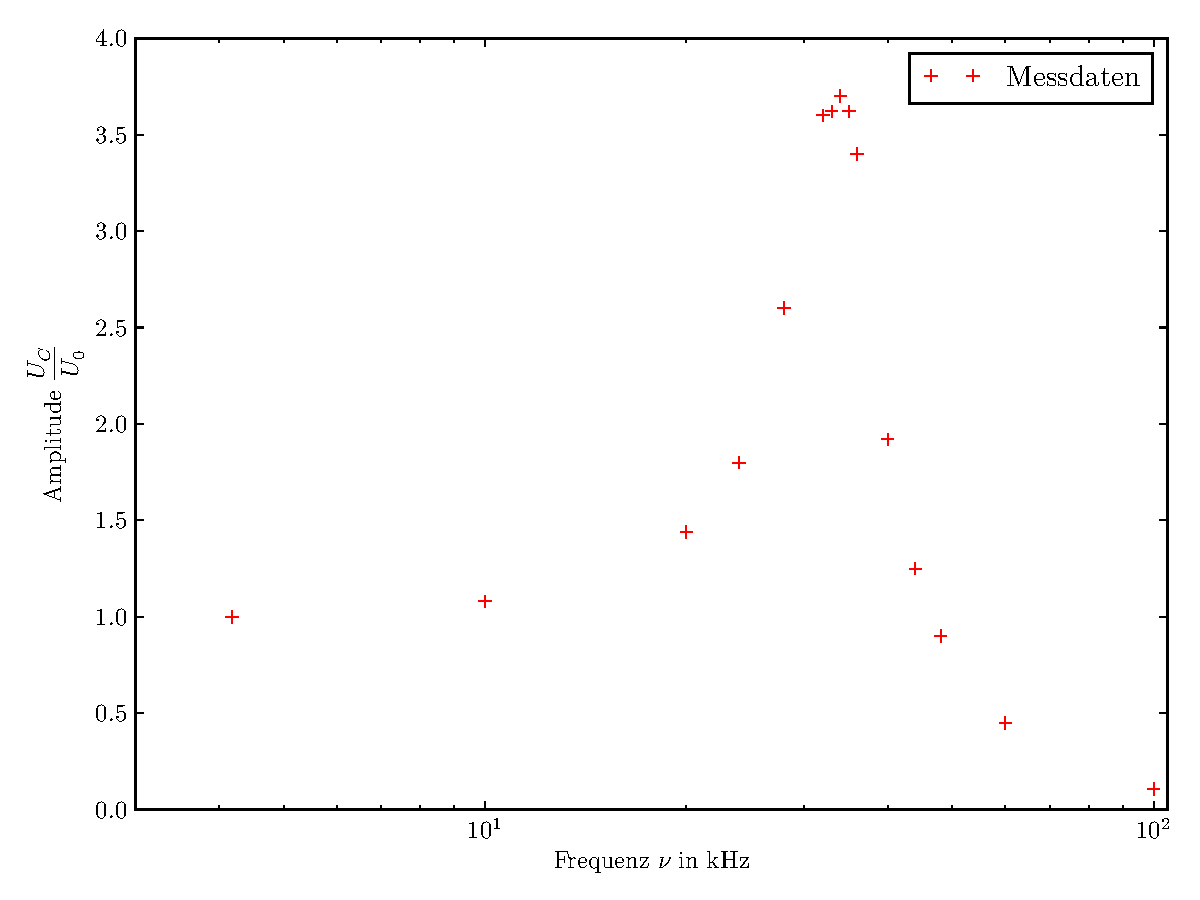
\includegraphics[width=\textwidth]{Plot2.pdf}
  \caption{Halblogarithmische Darstellung des Spannungsverlaufes.}
  \label{fig:plot2}
\end{figure}
\begin{figure}[htb]
  \centering
  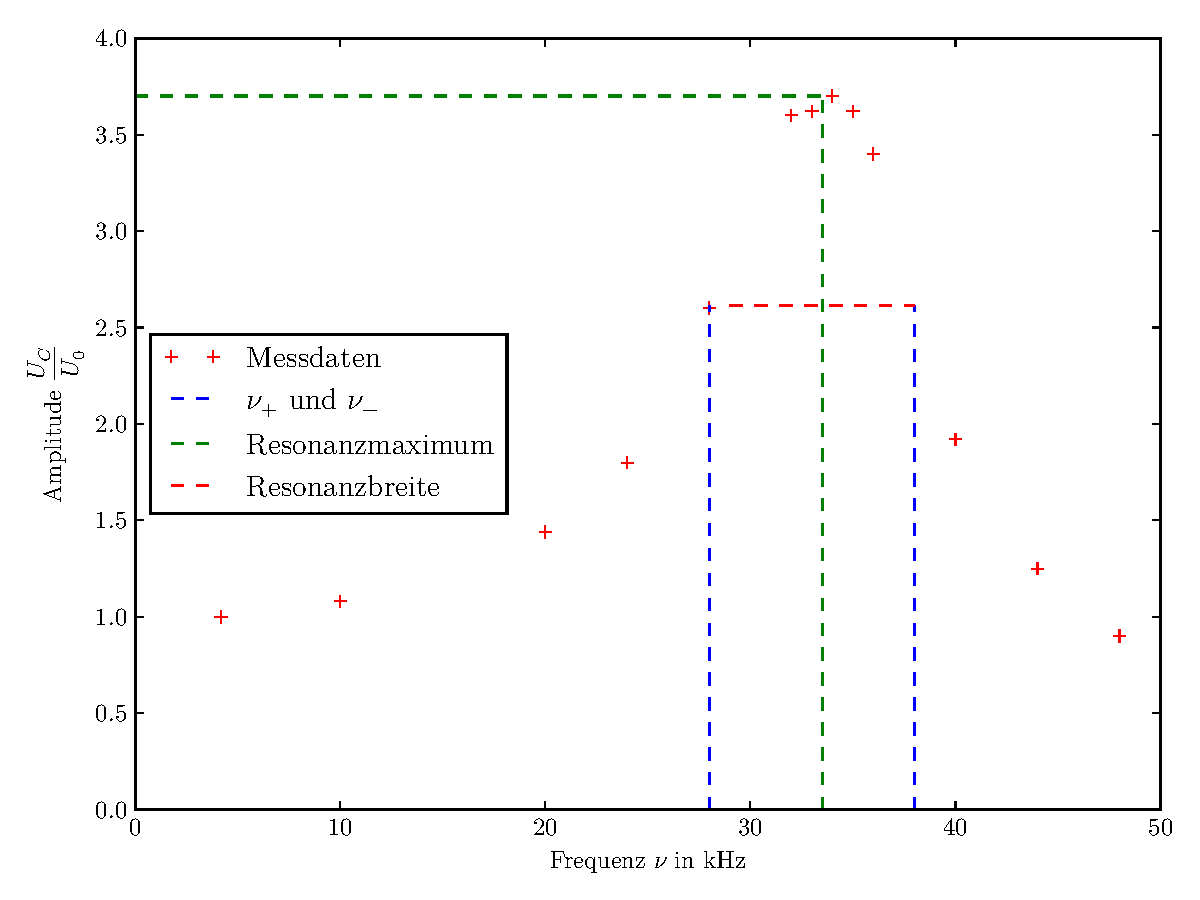
\includegraphics[width=\textwidth]{Plot3.pdf}
  \caption{Lineare Darstellung des Spannungsverlaufes.}
  \label{fig:plot3}
\end{figure}
\clearpage
Mit den Werten für $\increment t$ und $\nu$ aus Tabelle \ref{tab:messwerte2}
lässt sich die eigentliche Phasenverschiebung $\phi$ nach
\begin{equation}
  \phi = \frac{\increment t}{T} \cdot \SI{360}{\degree} = \increment t \cdot \nu \cdot \SI{360}{\degree}
\end{equation}
bzw.
\begin{equation}
  \phi = \frac{\increment t}{T} \cdot 2\pi = \increment t \cdot \nu \cdot 2\pi
\end{equation}
bestimmen. Die Ergebnisse davon stehen in Tabelle \ref{tab:phase}
\begin{table}
  \centering
  \caption{Phasenverschiebung.}
  \label{tab:phase}
  \sisetup{table-format=3.2}
  \begin{tabular}{S S S[table-format=1.3]}
    \toprule
    {Frequenz $\nu$ des}\\ {Generators in $\si{\kilo\hertz}$} & {$\phi \,/\, \si{\degree}$} & {$\phi$ in rad}\\
    \midrule
    4.183 & 1.87 & 0.033\\
    10 & 4.72 & 0.082\\
    20 & 10.08 & 0.176\\
    24 & 14.17 & 0.247\\
    28 & 23.08 & 0.403\\
    32 & 50.8 & 0.887\\
    33 & 77.22 & 1.348\\
    34 & 90.58 & 1.581\\
    35 & 104.58 & 1.825\\
    36 & 116.64 & 2.036\\
    40 & 144 & 2.513\\
    44 & 156.82 & 2.737\\
    48 & 161.57 & 2.82\\
    60 & 170.64 & 2.978\\
    100 & 194.4 & 3.393\\
    \bottomrule
  \end{tabular}
\end{table}\\
Diese werden nun ebenfalls einmal halblogarithmisch (Abbildung \ref{fig:plot4})
und einmal linear (Abbildung \ref{fig:plot5}) aufgetragen. Der Letzte Wert liegt
über der Grenze von $\pi$. Daher wird er in den Graphen vernachlässigt.
Geometrisch werden nun die Frequenzen $\nu_0$, $\nu_1$ und $\nu_2$ bestimmt.
\begin{align}
  \nu_0 = \SI{34.1}{\kilo\hertz} & &\nu_1 = \SI{30.8}{\kilo\hertz} & &\nu_2 = \SI{38.8}{\kilo\hertz}.
\end{align}
Mit den Formeln \eqref{eqn:phasepi2} und \eqref{eqn:phase134pi} ergeben sich folgende
theoretischen Werte:
\begin{align}
  \nu_0 = \SI{34.6}{\kilo\hertz} & &\nu_1 = \SI{30.8}{\kilo\hertz} & &\nu_2 = \SI{38.8}{\kilo\hertz}.
\end{align}
\begin{figure}[htb]
  \centering
  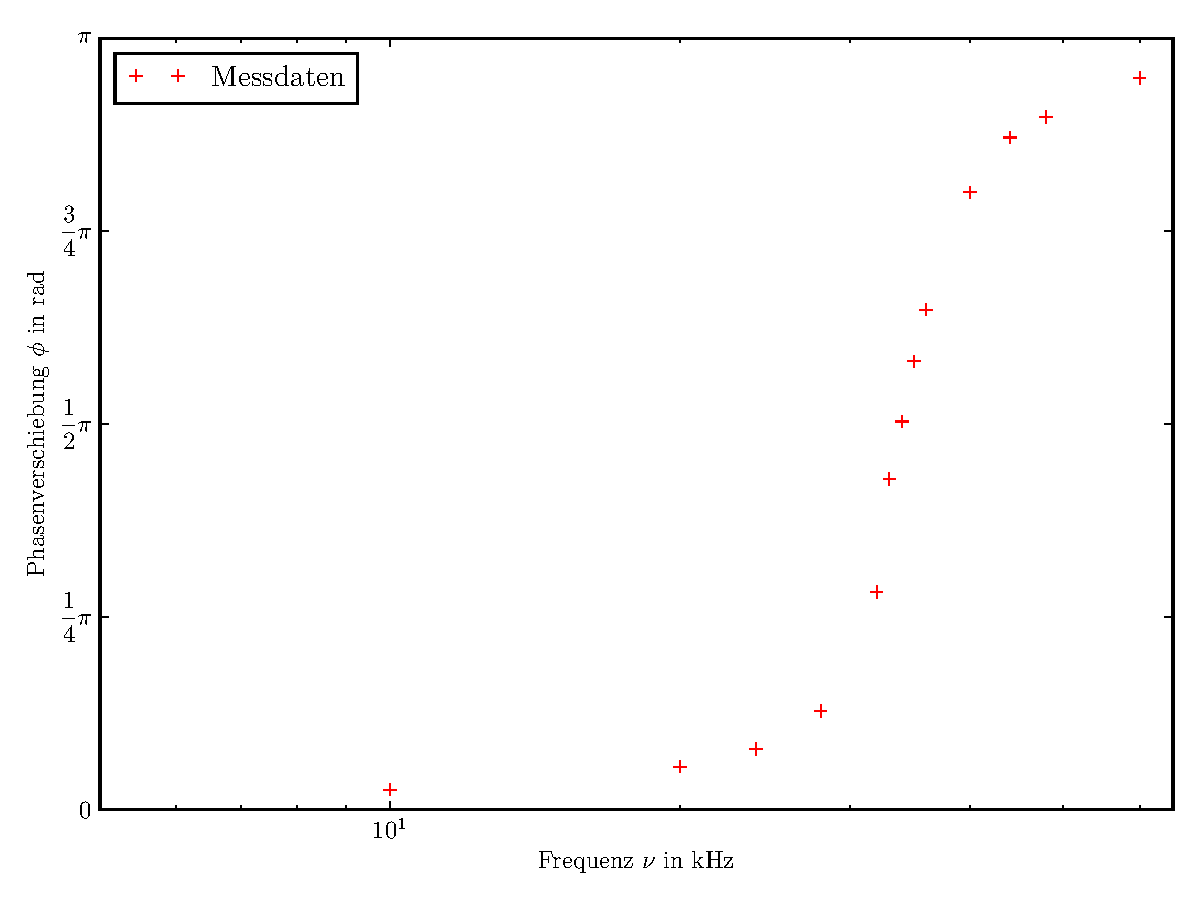
\includegraphics[width=\textwidth]{Plot4.pdf}
  \caption{Halblogarithmische Darstellung der Phase.}
  \label{fig:plot4}
\end{figure}
\begin{figure}[htb]
  \centering
  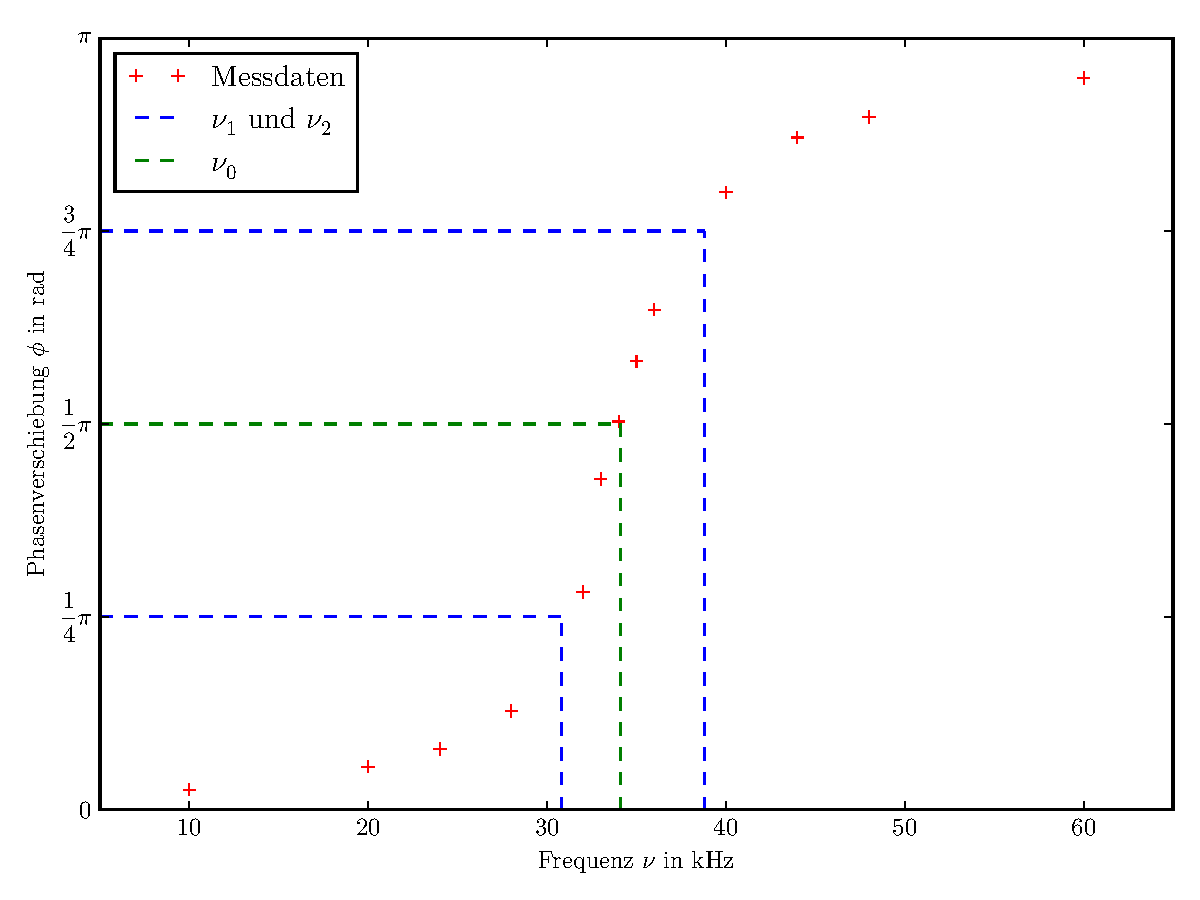
\includegraphics[width=\textwidth]{Plot5.pdf}
  \caption{Lineare Darstellung der Phase.}
  \label{fig:plot5}
\end{figure}
\section{Diskussion}
\label{sec:diskussion}
\begin{table}
  \centering
  \caption{Ergebnisse, Theoriewerte und relative Abweichung.}
  \label{tab:ergebnisse}
  \sisetup{table-format=4.3}
  \begin{tabular}{S[table-format=1.1] S S S[table-format=2.1]}
    \toprule
    & {Theoretischer Wert} & {Ergebniss} & {relative Abweichung}\\
    \midrule
    $T_\mathup{ex}$ & $\SI{420}{\micro\second}$ & $\SI{179(6)}{\micro\second}$ & $\SI{57.4}{\percent}$\\
    $R_\mathup{eff}$ & $\SI{48.1}{\ohm}$ & $\SI{113(4)}{\ohm}$ & $\SI{135}{\percent}$\\
    $R_\mathup{ap}$ & $\SI{4390(9)}{\ohm}$ & $\SI{3600}{\ohm}$ & $\SI{18}{\percent}$\\
    ${\nu_\mathup{res}}$ & $\SI{34.1}{\kilo\hertz}$ & $\SI{33.5}{\kilo\hertz}$ & $\SI{1.8}{\percent}$\\
    $q$ & 4.3 & 3.7 & $\SI{14}{\percent}$\\
    ${\nu_+ - \nu_-}$ & $\SI{8}{\kilo\hertz}$ & $\SI{10}{\kilo\hertz}$ & $\SI{25}{\percent}$\\
    ${\nu_0}$ & $\SI{34.6}{\kilo\hertz}$ & $\SI{34.1}{\kilo\hertz}$ & $\SI{1.4}{\percent}$\\
    ${\nu_1}$ & $\SI{30.8}{\kilo\hertz}$ & $\SI{30.8}{\kilo\hertz}$ & $\SI{0}{\percent}$\\
    ${\nu_2}$ & $\SI{38.8}{\kilo\hertz}$ & $\SI{38.8}{\kilo\hertz}$ & $\SI{0}{\percent}$\\
    \bottomrule
  \end{tabular}
\end{table}
In Tabelle \ref{tab:ergebnisse} stehen die Ergebnisse der Auswertung zusammen mit
den theoretischen Werten. Die Abweichung bei der Abklingdauer lässt sich auf den
Unterschied bei den effektiven Widerständen zurück führen. Dieser wiederum kommt
wahrscheinlich durch nicht bedachte Leitungswiderstände oder z.B. den Innenwiderstand
des Generators zustande. Selbige Gründe sind voraussichtlich für den Unterschied
bei dem Widerstand für den aperiodischen Grenzfall verantwortlich. Zudem kam es
wahrscheinlich zu Abweichungen durch Ungenauigkeiten an dem Verstellrädchen.
Die gemessene Resonanzfrequenz befindet sich relativ nah an dem theoretischen Wert.
Der etwas kleinere gemessene Wert bei der Güte kann ebenfalls mit dem Unterschied
zwischen eingebautem und effektivem Widerstand begründet werden.
Da Formel \eqref{eqn:breite} nur eine Näherung darstellt, weicht der gemessene
Wert von $\nu_+ - \nu_-$ etwas vom Theoretischen ab. Die restlichen gemessenen Werte für $\nu_0$,
$\nu_1$ und $\nu_2$ passen sehr gut zu den theoretischen Werten.
\clearpage
\nocite{*}
\printbibliography

\end{document}
